
%(BEGIN_QUESTION)
% Copyright 2013, Tony R. Kuphaldt, released under the Creative Commons Attribution License (v 1.0)
% This means you may do almost anything with this work of mine, so long as you give me proper credit

In this safety shutdown system, a programmable logic controller (PLC) monitors inputs coming from various switches located on a large motor-driven gas compressor system, and trips the compressor off (shuts off power to the motor's contactor coil) if any of these conditions becomes dangerous.

$$\includegraphics[width=15.5cm]{i03125x01.eps}$$

Noting the status of the LEDs on the discrete input card of the PLC while the compressor is running as it should, identify what you would have to do to electrically simulate the following trip conditions (i.e. make the PLC ``think'' that a dangerous condition existed when in fact one did not):

\begin{itemize}
\item{} Abnormal oil pressure
\item{} Abnormal oil level
\item{} Abnormal coolant temperature
\item{} Abnormal coolant pressure
\item{} High axial vibration
\item{} High radial vibration
\item{} Overcurrent condition detected
\end{itemize}

\underbar{file i03125}
%(END_QUESTION)





%(BEGIN_ANSWER)

We see the LED energized for channel {\tt IN1} on the PLC input card, telling us that the oil pressure switch is in the {\it closed} state while the compressor is running as it should.  This means we need to force that input to {\it de-energize} in order to make the PLC ``think'' there is an oil pressure problem.  Introducing a break into the circuit for this input channel will simulate a trip condition.

\vskip 10pt

We see the LED de-energized for channel {\tt IN4} on the PLC input card, telling us that the oil level switch is in the {\it open} state while the compressor is running as it should.  This means we need to force that input to {\it energize} in order to make the PLC ``think'' there is an oil level problem.  Jumpering power to the input channel will simulate a trip condition.

\vskip 10pt

We see the LED de-energized for channel {\tt IN2} on the PLC input card, telling us that the coolant temperature switch is in the {\it open} state while the compressor is running as it should.  This means we need to force that input to {\it energize} in order to make the PLC ``think'' there is a coolant temperature problem.  Jumpering power to the input channel will simulate a trip condition.

\vskip 10pt

We see the LED de-energized for channel {\tt IN3} on the PLC input card, telling us that the coolant pressure switch is in the {\it open} state while the compressor is running as it should.  This means we need to force that input to {\it energize} in order to make the PLC ``think'' there is a coolant pressure problem.  Jumpering power to the input channel will simulate a trip condition.

\vskip 10pt

We see the LED energized for channel {\tt IN5} on the PLC input card, telling us that the axial vibration switch is in the {\it closed} state while the compressor is running as it should.  This means we need to force that input to {\it de-energize} in order to make the PLC ``think'' there is an axial vibration problem.  Introducing a break into the circuit for this input channel will simulate a trip condition.

\vskip 10pt

We see the LED energized for channel {\tt IN7} on the PLC input card, telling us that the radial vibration switch is in the {\it closed} state while the compressor is running as it should.  This means we need to force that input to {\it de-energize} in order to make the PLC ``think'' there is an radial vibration problem.  Introducing a break into the circuit for this input channel will simulate a trip condition.

\vskip 10pt

We see the LED de-energized for channel {\tt IN6} on the PLC input card, telling us that the protective relay contact is in the {\it open} state while the compressor is running as it should.  This means we need to force that input to {\it energize} in order to make the PLC ``think'' there is an overcurrent problem.  Jumpering power to the input channel will simulate a trip condition.

%(END_ANSWER)





%(BEGIN_NOTES)



\vskip 20pt \vbox{\hrule \hbox{\strut \vrule{} {\bf Virtual Trip-testing} \vrule} \hrule}

This question is a good candidate for a ``Virtual Trip-testing'' exercise.  Presenting the diagram to students, you pose an assignment whereby students must figure out how to test some component of this system to check that it will operate as intended to shut down the system in an abnormal (trip) condition, with some realistic limitation (e.g. power cannot be shut off to the load).  Students then propose various methods for executing the test.  Your job is to determine whether or not their proposed tests will achieve the desired result(s).

During and after the exercise, it is good to ask students follow-up questions such as:

\begin{itemize}
\item{} Where might our planned test strategy go wrong?  In other words, what thing(s) might happen to foil our test, either to invalidate the results or to not honor the stated limitation(s)?
\item{} Suppose the limitation were different.  How would this affect our ability to carry out the test?
\item{} Is the last test strategy best one we could execute?
\end{itemize}


%INDEX% Safety, shutdown system: trip testing

%(END_NOTES)


